\documentclass{beamer}
\usepackage{graphicx}
\usepackage{tikz}
\usetikzlibrary{shapes,arrows}
\usepackage{tikz}
%\usecolortheme{seahorse}
  \setbeamertemplate{footline}[page number]
\usepackage{multirow}
\setbeamertemplate{navigation symbols}{}
\setbeamertemplate{frametitle}[default][center]
\setbeamerfont{frametitle}{shape=\scshape}
\usepackage{color}

\usepackage{csquotes}

\usepackage{xcolor}

\usepackage[flushleft]{threeparttable}

{\title{\textsc{Econ 352 - Money, Inflation, and Banking: A Deeper Look} \\ \tiny (See Williamson Ch. 18)}
\author{Trevor S. Gallen}
\date{}
\begin{document}
\renewcommand*{\inserttotalframenumber}{\pageref{lastframe}}


\setbeamertemplate{caption}{\raggedright\insertcaption\par}

\begin{frame}
\titlepage
\end{frame}

\begin{frame}
\frametitle[alignment=center]{Introduction}
\begin{itemize}
\item We had a simple model of money markets so far
\bigskip
\item This chapter looks to break into finance a little bit more
\bigskip
\item So far, banks didn't really play a role!
\bigskip
\item We'll look at the Diamond-Dybvig bank model
\begin{itemize}
\item Dybvig, Diamond, and Ben Bernanke all won Econ Nobel  in 2022 for work on this topic!
\end{itemize}
\bigskip
\item First, we'll talk about some history of money \& barter
\end{itemize}
\end{frame}


\begin{frame}
\frametitle[alignment=center]{Alternative Forms of Money-Commodity}
\begin{itemize}
\item Historically, we had commodity money (Greeks, Romans)
\bigskip
\item Coin in gold, silver, copper
\bigskip
\item Big issues:  chipping, sweating, plugging
\bigskip
\item Process is expensive (mining, etc)
\bigskip
\item Held up, with periodic big problems, for millenia
\end{itemize}
\end{frame}

\begin{frame}
\frametitle[alignment=center]{Private Bank Notes}
\begin{itemize}
\item In U.S. 1837-1863, banks would produce their own currencies that bank would redeem
\bigskip
\item Chicago bank might be trusted around Chicago, but not around New York, would take notes at a discount
\bigskip
\item Big process of verification
\bigskip
\item Also a lot of fraud \& failures!
\end{itemize}
\end{frame}

\begin{frame}
\frametitle[alignment=center]{Fiat Money}
\begin{itemize}
\item Our current system!
\bigskip
\item Government prints pieces of paper, promises future demand via taxes
\bigskip
\item Requiring money for taxes gives it intrinsic value, not just hopes others will accept it
\bigskip
\item If govt requires that 10\% of my budget be paid in dollars, I (and others) demand dollars, and will give up real assets for them!
\bigskip
\item Sometimes people just say ``only held up by faith," even if wrong
\end{itemize}
\end{frame}

\begin{frame}
\frametitle[alignment=center]{Transaction Deposits at Private Banks}
\begin{itemize}
\item People don't just use dollars!
\bigskip
\item Now, we send money digitally between banks, cleared through an interbank transaction (FedWire)
\bigskip
\item We wouldn't include credit cards--credit created is not money, it's an IOU by a private entity
\end{itemize}
\end{frame}


\begin{frame}
\frametitle[alignment=center]{Unusual Money-Yap}
\begin{itemize}
\item In Micronesia, they used large stones--1 ft to 12 ft long
\bigskip
\item Not from island, quarried far away (hard to create)
\bigskip
\item Money was frequently not moved physically, but just reassigned (small population knew who owned what)
\bigskip
\item ``Money is memory"
\bigskip
\item Similarly, historical IOU's:  playing cards in ``New France" (Quebec)
\end{itemize}
\end{frame}

\begin{frame}
\frametitle[alignment=center]{Money and Coincidence of Wants}
\begin{itemize}
\item Money helps solve an issue in Barter
\bigskip
\item Person 1 wants Person 2's production, Person 2 want's Person C's production, and Person C wants Person A's production
\bigskip
\item Hard to find person who wants what you have!
\bigskip
\item How can P1, P2 and P3 all solve this problem?
\bigskip
\item If P2 accepts P1's production, can then trade to P3, solves situation
\bigskip
\item Fiat money does too--if we all expect one another to accept it, we'll all be willing to accept it
\end{itemize}
\end{frame}

\begin{frame}
\frametitle[alignment=center]{Absence of Double-Coincidence of Wants}
\begin{figure}
\centering
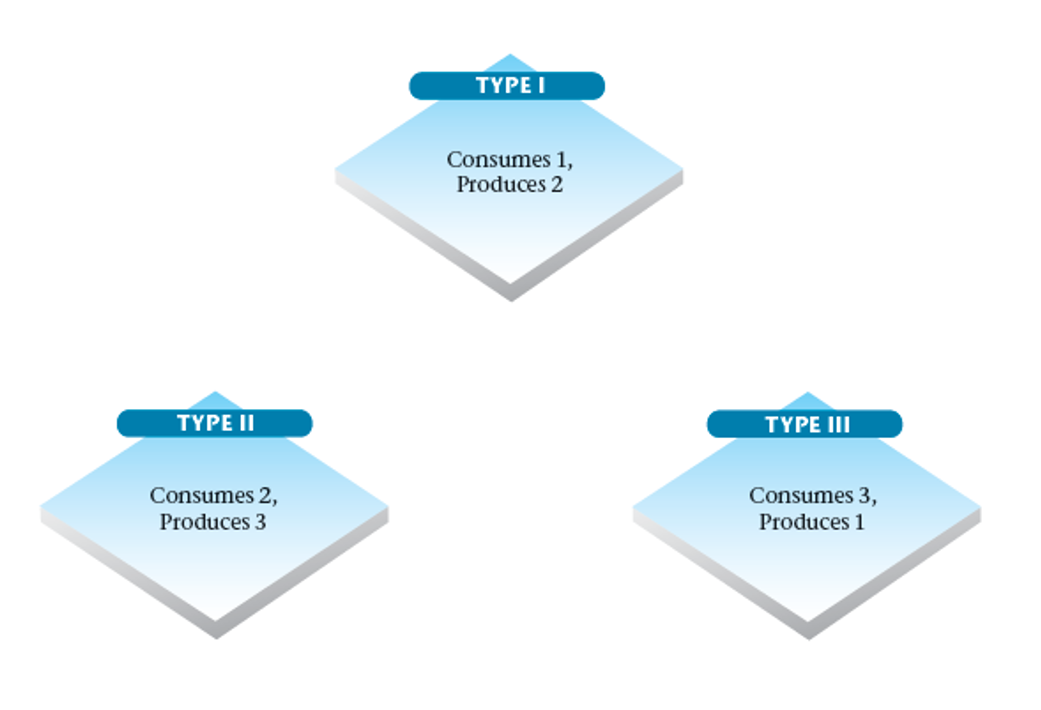
\includegraphics[scale=0.6]{Figures/W_Fig_18pt1.png}
\end{figure}
\end{frame}

\begin{frame}
\frametitle[alignment=center]{Good 1 is Commodity Money}
\begin{figure}
\centering
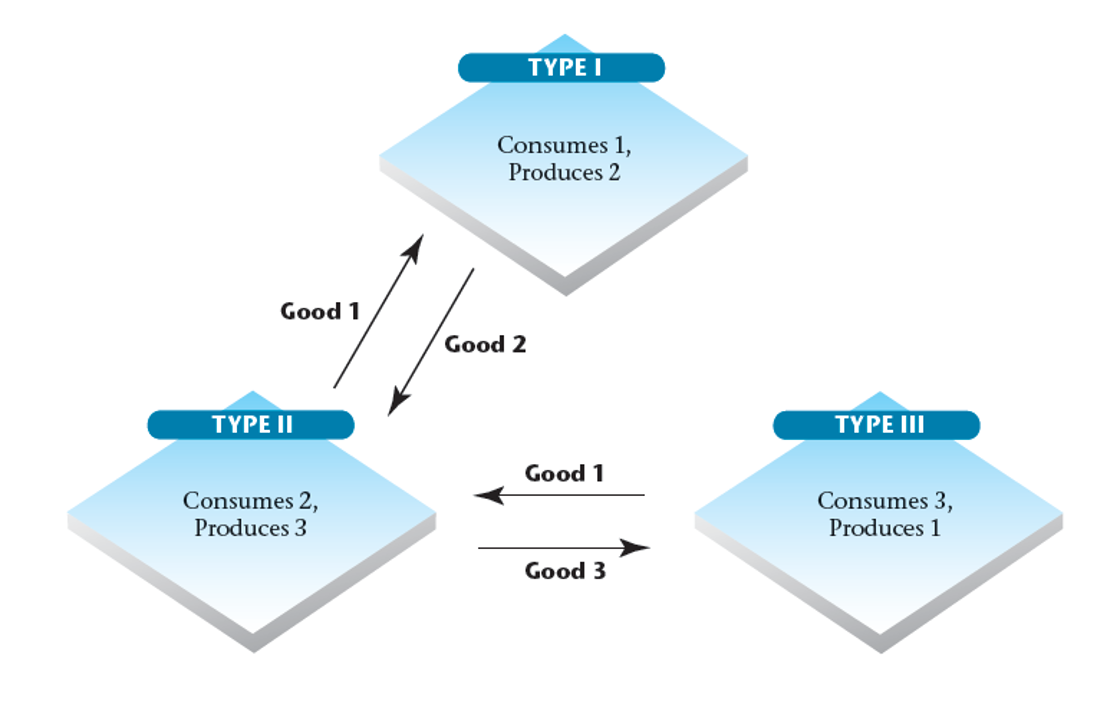
\includegraphics[scale=0.6]{Figures/W_Fig_18pt2.png}
\end{figure}
\end{frame}

\begin{frame}
\frametitle[alignment=center]{Fiat Money Solves}
\begin{figure}
\centering
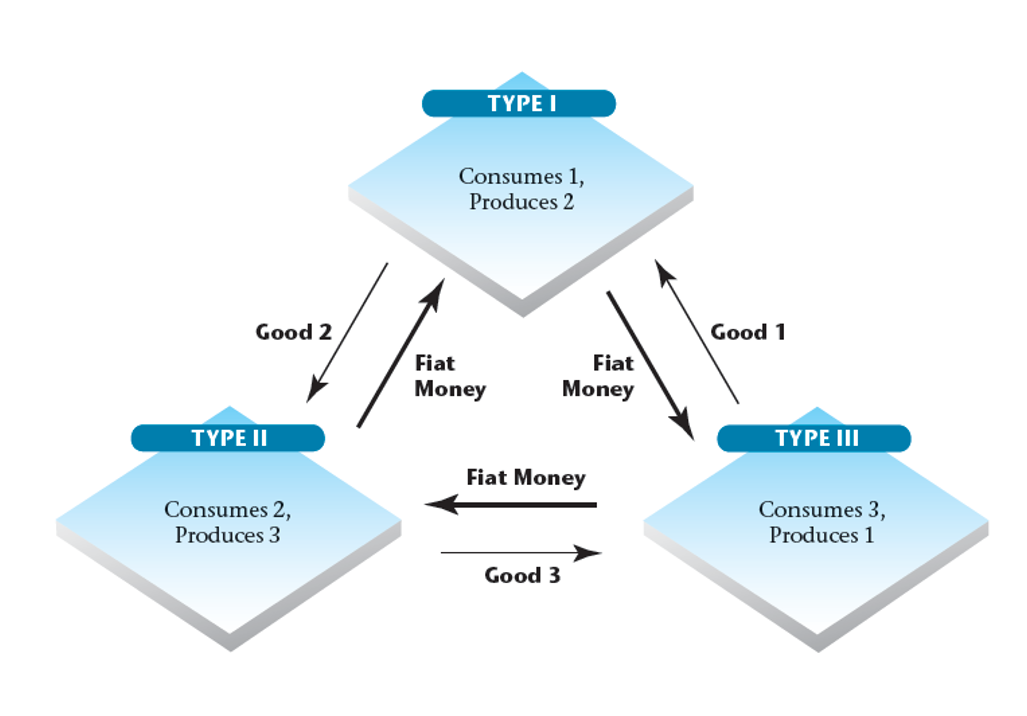
\includegraphics[scale=0.6]{Figures/W_Fig_18pt3.png}
\end{figure}
\end{frame}


\begin{frame}
\frametitle[alignment=center]{Long-Run Inflation in the Monetary Intertemporal Model}
\begin{itemize}
\item Previously we had a model in which money was neutral: changes in the level of money have no effects
\smallskip
\item But what about changes in the \emph{growth rate} of money?
\smallskip
\item Assume that money grows at a constant rate: $M'=(1=x)M$
\smallskip
\item And we have money demand:  $M=PL(Y,r+i)$
\smallskip
\item So:
$$\frac{M'}{M}=\frac{P'L(Y',r'+i')}{PL(Y,r+i)}$$
\item In equilibrium, we have:
$$\frac{M'}{M}=\frac{P'}{P}$$
\item Money growth determines inflation:
$$i=x$$
\end{itemize}
\end{frame}


\begin{frame}
\frametitle[alignment=center]{Summarizing Idea}
\begin{itemize}
\item When $M'/M$ increases, then $P'/P$ increases, so inflation $i$ increases.
\bigskip
\item This increases the nominal interest rate: if we hold cash today to buy things tomorrow, consuming is now more expensive (or real wage tradeoff is lower)
\bigskip
\item So leisure more today!
\bigskip
\item Labor supply shifts in, output supply and demand shift in
\bigskip
\item $r$ could change, but we assume roughly cancel, so $r$ constant
\bigskip
\item \emph{Changes} in money growth not neutral: ``money may be neutral (changes in level doesn't matter), but isn't superneutral (changes in growth rate matter)"
\end{itemize}
\end{frame}


\begin{frame}
\frametitle[alignment=center]{Increase in Money Growth Rate}
\begin{figure}
\centering
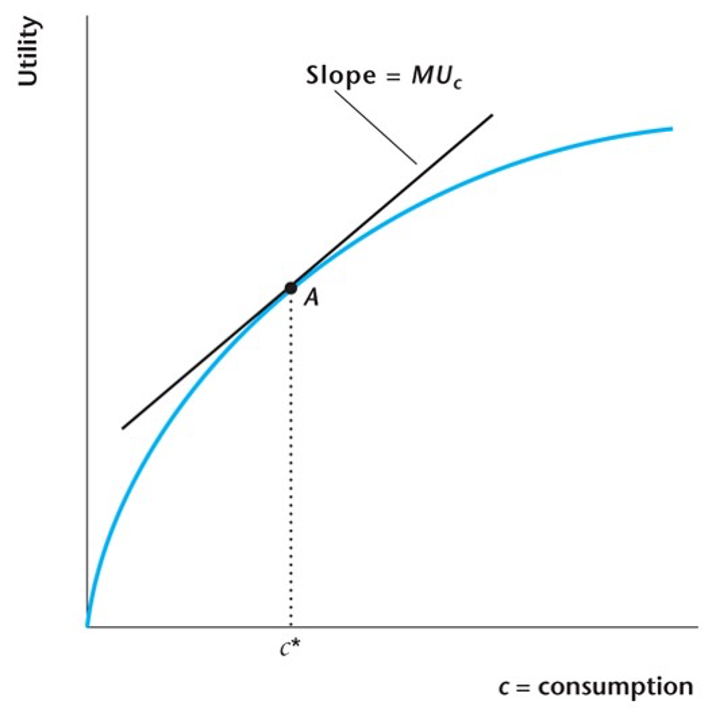
\includegraphics[scale=0.75]{Figures/W_Fig_18pt5.png}
\end{figure}
\end{frame}

\begin{frame}
\frametitle[alignment=center]{Friedman Rule}
\begin{itemize}
\item The MRS summarizes the slope of utility, while MRT summarizes budget constraint/tradeoff
\bigskip
\item Equilibrium was where:
$$MRS_{l,C}=MRT_{l,C}$$
\item We had that for firmst, $MRT_{l,c}=w$, so:
$$MRS_{l,C}=w$$
\item Which becomes:
$$MRS_{l,C}=\frac{MRT_{l,C}}{1+R}$$
\item This is bad!  Good means $MRS=MRT$, but there's an inefficient wedge due to nominal interest rates
\bigskip
\item Government can fix by setting $R=1$
\bigskip
\item $R=r+i$, so $i=-r$ is best
\bigskip
\item Idea: cash is causing inefficiencies, but can solve by setting return to cash same as return on bonds
\end{itemize}
\end{frame}

\begin{frame}
\frametitle[alignment=center]{Financial Intermediation}
\begin{itemize}
\item Four important properties of assets:
\bigskip
\begin{itemize}
\item Rate of return:  when you purchase an asset, you get its value next period plus any dividends:
$$r_t^a=\frac{q_{t+1}+d}{q_t}-1$$
\item Risk:  dispersion in returns (less volatile is better!)
\bigskip
\item Maturity:  how long is your loan for? (shorter is better!)
\bigskip
\item Liquidity: how quickly can you sell the asset? (more liquid is better!)
\end{itemize}
\end{itemize}
\end{frame}

\begin{frame}
\frametitle[alignment=center]{Financial Intermediation}
\begin{itemize}
\item Financial Intermediaries:
\bigskip
\begin{itemize}
\item Borrow from one group of economic agents and lends to another
\bigskip
\item Group of agents it borrows from is large, and so is group it lends to (diversified)
\bigskip
\item Transforms assets:  borrows under different terms than it lends
\bigskip
\item Processes information
\end{itemize}
\item All sorts of intermediaries!  Mutual funds, insurance companies, banks
\end{itemize}
\end{frame}

\begin{frame}
\frametitle[alignment=center]{Financial Intermediation}
\begin{itemize}
\item Some issues in lending without financial intermediation:
\bigskip
\begin{itemize}
\item Matching borrowers with lenders is costly in time and effort
\bigskip
\item The ultimate lenders may not be skilled at evaluating credit risks
\bigskip
\item Because several lenders would often be required to fund any one borrower, there would be replication of costs required to evaluate credit risk
\bigskip
\item Because lenders economize on information costs by lending to few borrowers,  lending is risky
\bigskip
\item Loans tend to be illiquid
\bigskip
\item Loans tend to have longer maturities than lenders would like
\end{itemize}
\bigskip
\item Financial system tries to fix these problems
\end{itemize}
\end{frame}




\begin{frame}
\frametitle[alignment=center]{Note!}
\begin{itemize}
\item Williamson has a treatment of Diamond-Dybvig
\bigskip
\item I'm going to take my treatment from Doepke, Lehnert, and Sellgren (1999) Ch. 17.4
\bigskip
\item Both give same idea, but I love Doepke, Lehnert and Sellgren's treatment!
\end{itemize}
\end{frame}


\begin{frame}
\frametitle{The basic idea}
\begin{itemize}
\item<1-> Banks are going to do something good.  They'll:
\bigskip
\begin{itemize}
\item<2-> Take money (deposits)
\bigskip
\item<2-> Allow you to withdraw it at any time (liquidity)
\bigskip
\item<2-> Invest it for you and pay you for the right to loan it out (interest)
\bigskip
\end{itemize}
\item<3-> But there will be a big problem...what?
\bigskip
\item<4-> Because of how banks are structured, they'll be vulnerable to \textbf{bank runs}
\end{itemize}
\end{frame}

\begin{frame}
\frametitle{Diamond and Dybvig}
\begin{itemize}
\item<1-> Diamond and Dybvig:
\blockquote{Bank runs are a common feature of the extreme crises that have played a prominent role in monetary history. During a bank run, depositors rush to withdraw their deposits because they expect the bank to fail. In fact, the sudden withdrawals can force the bank to liquidate many of its assets at a loss and to fail. In a panic with many bank failures, there is a disruption of the monetary system and a reduction in production.}
\item<2-> The point: there are multiple equilibria.  If everyone thinks the bank will fail, it fails.  If people don't think it is fine, it will be.
\bigskip
\item<3-> We'll tell a highly stylized story about turnips now.  
\end{itemize}
\end{frame}

\begin{frame}
\frametitle{Key To Bank Runs and Financial Crises???}
\begin{figure}
\centering

\includegraphics[scale=0.05]{Figures/turnip.jpg}
\end{figure}
\end{frame}

\begin{frame}
\frametitle{Key To Bank Runs and Financial Crises???}
\begin{figure}
\centering

\includegraphics[scale=0.2]{Figures/turnip.jpg}
\end{figure}
\end{frame}

\begin{frame}
\frametitle{Key To Bank Runs and Financial Crises???}
\begin{figure}
\centering

\includegraphics[scale=0.85]{Figures/turnip.jpg}
\end{figure}
\end{frame}

\begin{frame}
\frametitle{A whole new world}
\begin{enumerate}
\item<1-> Our world starts off with a turnip technology: everything is turnips
\bigskip
\item<2-> Everyone starts off in period 0 with a turnip
\bigskip
\item<3-> They can all plant it (or give it to the bank to plant)
\bigskip
\item<4-> At the beginning of period 1, some proportion of the population $\theta$ finds out they'll die at the end of the period
\bigskip
\item<5-> Everyone can uproot their turnip and get 1 turnip back
\bigskip
\item<6-> At the beginning of period 2, all the turnips that are left grow to be $F>1$ turnips
\bigskip
\item<7-> If you're still alive, you can eat your turnip
\end{enumerate}
\end{frame}

\begin{frame}
\frametitle{Preferences}
\begin{itemize}
\item<1-> In this world everyone is perfectly patient (if alive).  Let:
\smallskip
\begin{itemize}
\item<2-> $c_1$ be consumption in period 1 
\smallskip
\item<2->  $c_2$ be consumption in period 2 
\smallskip
\item<3->  $\Theta$ be your ``type"
\smallskip
\begin{itemize}
\item<3->  $\Theta=1$ if you die in period 1
\smallskip
\item<3-> $\Theta=2$ if you die in period 2 
\end{itemize}
\end{itemize}
\item[]<4->  \ 
$$U(c_1,c_2,\Theta)=\left\{\begin{array}{ll}\log(c_1) & \text{if }\Theta=1 \\ Q\log(c_1+c_2) & \text{if }\Theta=2\end{array}\right\}$$
\item<4-> Where $1>Q>F^{-1}$, which will control how important it is to consume if you're the second type.
\item<5-> The point of these preferences is just to say:
\smallskip
\begin{itemize} 
\item<6-> ``People are have diminishing returns to consumption/are risk averse" 
\smallskip
\item<7->  ``The second type is willing to wait if it gains her anything"
\end{itemize}
\end{itemize}
\end{frame}

\begin{frame}
\frametitle{On your own}
\begin{itemize}
\item<1-> Imagine you're on your own in this world: what do you do?
\bigskip
\begin{enumerate}
\item<2-> Plant turnip in period 0
\bigskip
\item<3-> Enter period 1, find out type
\bigskip
\item<4-> If type 1 (die in period 1) then dig up turnip, eat 1 turnip, get $\log(1)$
\bigskip
\item<5-> If type 2 (die in period 2) then wait until period 2, dig up turnip, eat $F>1$ turnips, get $\log(F)$
\end{enumerate}
\item<7-> To put meat and bones on this, I'm going to say that $F=1.1$, and $\theta=0.5$, $1>Q>F^{-1}$ is, 0.98:
\bigskip
\item<8-> Then with probability $\theta$ you get utility $\log(1)=0$ and with probability $(1-\theta)$ you get utility $\log(1.1)=0.095$.  
\bigskip
\item<9-> On your own, you get expected utility:
$$\theta\cdot \log(1)+(1-\theta)\cdot\log(1.1)=0.5\cdot0+0.98 +0.5\cdot 0.095=0.046702$$
\end{itemize}
\end{frame}

\begin{frame}
\frametitle{Join together}
\begin{itemize}
\item<1-> Question:  can banks improve on this?  Can we gain by joining together?
\bigskip
\item<2-> Yes!  This is what insurance markets are for!
\bigskip
\item<3-> We could all pay a premium (give up our turnips) in period zero
\bigskip
\item<4-> If we find out we're type 1, insurance company digs up our turnip and a little of someone else's, pays us some amount greater than 1
\bigskip
\item<5-> If we find out we're type 2, insurance company will have some turnips left over, pays us some amount less than $F$ and greater than 1
\bigskip
\item<6-> We can all be better off by using insurance to smooth our consumption across states of the world
\end{itemize}
\end{frame}

\begin{frame}
\frametitle{Budget constraint of the insurance company}
\begin{itemize}
\item<1-> The insurance company will pay out $c_1^1$ to all individuals of type $1$ and $c_2^2$ to all individuals of type 2
\bigskip
\item<2-> Their budget constraint is, normalizing the population to 1,
$$\theta c_1^1 + \frac{(1-\theta)c_2^2}{F}=1$$
\bigskip
\item<3-> This is saying that I have 1 turnip: if I increase $c_1^1$ a little, I lose that whole amount (times the population weight).  If I increase $c_2^2$, I only have to leave $\frac{1}{F}$ turnips in the ground (times their population weight) in order to pay them.
\bigskip
\item<4-> If we wanted to graph to make the tradeoff clear, writing $c_1^1$ as a function of $c_2^2$, we get: 
$$c_1^1=\frac{1}{\theta}\left(1- \frac{(1-\theta)c_2^2}{F}\right)$$
\item<5-> Let's graph this, with $F=1.1$ and $\theta=0.5$
\end{itemize}
\end{frame}

\begin{frame}
\frametitle{Budget constraint example}
\begin{figure}
\centering
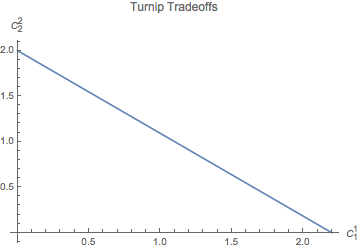
\includegraphics[scale=0.5]{Figures/turniptradeoff.png}
\end{figure}
\begin{itemize}
\item<2-> If you uproot the whole turnip and give it all to the half of the population that's type 1 in period 1, then they get 2 turnips each.
\smallskip 
\item<3-> If you uproot the whole $1.1$ turnip and give it all to the half of the population that's type 2 in period 2, then they get 2.2 turnips each.
\smallskip
\item<4-> Or you could do something in the middle
\end{itemize}
\end{frame}

\begin{frame}
\frametitle{Competition}
\begin{itemize}
\item<1->  What should the bank do?  Who should it pay?  Should it keep all the money?
\bigskip
\item<2-> If you don't do something that makes people as happy as possible, then another company will
\bigskip
\item<3-> Competition forces you to make the best decision for your population
\bigskip
\item<4-> Let's write down the utility maximization problem
\end{itemize}
\end{frame}

\begin{frame}
\frametitle{Insurance utility maximization}
$$\mathcal{L}(c_1^1,c_2^2,\lambda)=\theta \log(c_1^1)+(1-\theta)Q\log(c_2^2)+\lambda\left(1-\theta c_1^1-\frac{(1-\theta)c_2^2}{F}\right)$$
\begin{itemize}
\item Taking first order conditions, we get:
$$\begin{array}{lrcl}
\frac{\partial \mathcal{L}}{\partial c_1^1}: & \frac{\theta}{c_1^1}-\lambda\theta & = & 0 \\
\ \\
\frac{\partial \mathcal{L}}{\partial c_2^2}: & Q\frac{1-\theta}{c_2^2}-\lambda\frac{1-\theta}{F} & = & 0 \\
\ \\
\frac{\partial \mathcal{L}}{\partial \lambda}: & \theta c_1^1 + \frac{(1-\theta)c_2^2}{F}  & = & 1 \\
\end{array}$$
\bigskip
\item It's easy to solve these three equations for our three unknowns, $c_1^1$, $c_2^2$, and $\lambda$
\end{itemize}
\end{frame}

\begin{frame}
\frametitle{Insurance utility solution}
\begin{itemize}
\item Solving for $c_1^1$, $c_2^2$, and $\lambda$, we get:
$$c_1^1=\frac{1}{\theta+Q(1-\theta)}\ \ \ \ \ \ \ \ \ \ c_2^2=\frac{QF}{\theta+Q(1-\theta)}$$
\item<2-> Assuming that $1>Q>F^{-1}$ is, say, 0.98:
$$c_1^1=\frac{1}{0.5+0.98(1-0.5)}=1.\overline{01}$$
$$c_2^2=\frac{0.98\cdot 1.1}{\theta+0.98(1-\theta)}=1.0\overline{888}$$
\item<3-> Are people really better off?? They lose 0.011111 units if they're type 2 but only gain 0.010101 if they're type 1!
\item<4-> Recall we have to beat expected utility of 0.046702...let's see the expected utility
$$E_0(U(c_1^1,c_2^2,\Theta))=0.5\log(1.\overline{01})+0.5\log(1.0\overline{8})=0.046752$$
\item<5-> We did it!  Improved utility slightly.
\end{itemize}
\end{frame}

\begin{frame}
\frametitle{Insurance?}
\begin{figure}
\centering
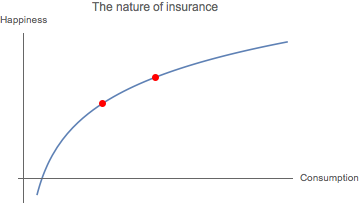
\includegraphics[scale=0.8]{Figures/Insurance_1.png}
\end{figure}
\end{frame}

\begin{frame}
\frametitle{Insurance?}
\begin{figure}
\centering
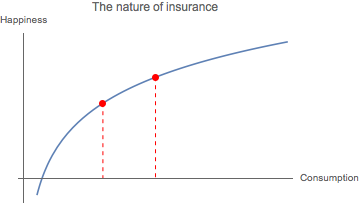
\includegraphics[scale=0.8]{Figures/Insurance_2.png}
\end{figure}
\end{frame}

\begin{frame}
\frametitle{Insurance?}
\begin{figure}
\centering
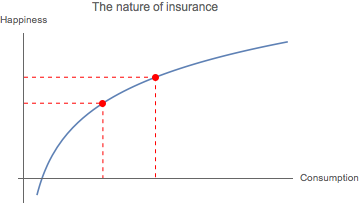
\includegraphics[scale=0.8]{Figures/Insurance_3.png}
\end{figure}
\end{frame}

\begin{frame}
\frametitle{Insurance?}
\begin{figure}
\centering
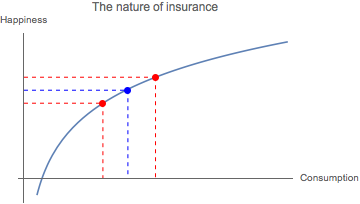
\includegraphics[scale=0.8]{Figures/Insurance_4.png}
\end{figure}
\end{frame}

\begin{frame}
\frametitle{Insurance?}
\begin{figure}
\centering
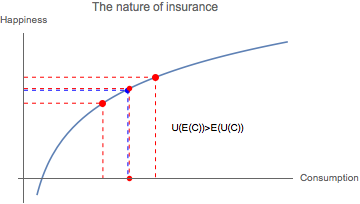
\includegraphics[scale=0.8]{Figures/Insurance_5.png}
\end{figure}
Utility of expected consumption preferred to expectation of utility.
\end{frame}


\begin{frame}
\frametitle{Insurance problem: summary}
\begin{itemize}
\item We have a problem in which people can invest and earn interest
\bigskip
\item But sometimes some people want their money now
\bigskip
\item Think of mortgages like planted turnips
\bigskip
\item Banks will allow people to withdraw whenever
\bigskip
\item People can benefit by participating in this ``insurance" system, where we're insuring your liquidity needs
\bigskip
\item Now we'll reframe this as a bank problem, but with one difference (what?)
\bigskip
\begin{itemize}
\item People can withdraw at any time! (No proof of type)
\end{itemize}
\end{itemize}
\end{frame}

\begin{frame}
\frametitle{Bank problem}
\begin{itemize}
\item Banks have the same problem as insurance companies, with a small twist:
\bigskip
\begin{enumerate}
\item They'll make promises in period 0 about how much you can receive if you withdraw in period 1 or period 2
\bigskip
\item They then have to keep those promises no matter how many people actually do withdraw in period 1
\end{enumerate}
\bigskip
\item The point:
\bigskip
\begin{itemize}
\item If too many people withdrew in period 1, then there would be nothing left in period 2!
\bigskip
\item If I fear too many people are going to withdraw in period 1, then I'll withdraw in period 1 even if I'm of type 2
\bigskip
\end{itemize}
\item Bank run!
\end{itemize}
\end{frame}

\begin{frame}
\frametitle{Bank problem}
\begin{itemize}
\item Banks face the same basic problem: choose an interest rate $r_1$ for type 1 and then whoever withdraws in period 2 gets the rest:
$$c_1^1=1+r_1$$
$$c_2^2=F\frac{1-\theta(1+r_1)}{1-\theta}$$
\item If for some reason $\theta$, the proportion that withdraw in period 1, is very high, then $c_2^2$ goes down.
\bigskip
\item If $c_2^2$ ever slips below $c_1^1$, then all the type 2's should run on the bank.
\bigskip
\item How should a bank choose $r_1$?
\bigskip
\item Maximize utility
\end{itemize}
\end{frame}

\begin{frame}
\frametitle{Bank maximization problem}
\begin{itemize}
\item Banks must maximize consumer expected utility, plugging in for $c_2^2$:
$$\theta\log(1+r_1)+(1-\theta)Q\log\left(F\frac{1-\theta(1+r)}{1-\theta}\right)$$
\item You can notice that this is the exact same problem as the insurance company faced, with $1+r_1=c_1$ and the budget constraint plugged in:
\bigskip
\item Consequently, it has the same maximization solutions: 
$$1+r_1=\frac{1}{\theta+Q(1-\theta)}$$
\item The bank chose the interest rate so everything is exactly the same as the insurance problem.
\bigskip
\item If all goes according to plan, type 1 will get $1.0\overline{1}$ and type 2 will get $1.0\overline{8}$
\bigskip
\item Type 2's won't want to run on the bank if nobody else is running on the bank, because they get more if they wait
\bigskip
\item But...
\end{itemize}
\end{frame}


\begin{frame}
\frametitle{Bank runs}
\begin{itemize}
\item What if for some reason I fear that too many people are withdrawing?  
\smallskip
\item Bank pays them out and I get the residual.  I should get $1.0\overline{8}$ if 50\% of population withdraws
\smallskip
\item What if 80\% withdraws?  Then I only get 
$$c_2^2=F\frac{1-\theta(1+r)}{1-\theta}=1.1\frac{1-0.6\cdot 1.0\overline{1}}{1-0.6}=1.05$$
\item Then I don't want to run
\smallskip
\item What if 89\% withdraws?  Then I get:
$$c_2^2=F\frac{1-\theta(1+r)}{1-\theta}=1.1\frac{1-0.89\cdot 1.0\overline{1}}{1-0.89}=1.001$$
\item If I fear that 89\% of the population should withdraw, then I'll withdraw too!
\smallskip
\item That means that (say) 90\% of the population is withdrawing, the heat is turned up for others who aren't withdrawing
\smallskip
\item Self-fulfilling Bank run!
\end{itemize}
\end{frame}

\begin{frame}
\frametitle{Bank runs: the story}
\begin{itemize}
\item If everyone is doing what they're supposed to, then there's no problem, everyone is happier and the economy is better than if there were no banks
\bigskip
\item But if I \emph{fear} too many people are withdrawing at once, then I should withdraw, creating a self-fulfilling bank run
\bigskip
\item This happens because banks make promises that they are able to keep only when people think they're able to keep them
\bigskip
\item Pro and con of banks:
\begin{itemize}
\item On the one hand, they improve utility
\bigskip
\item On the other hand, they're vulnerable to bank runs
\end{itemize}
\item Is there a way to avoid bank runs?
\end{itemize}
\end{frame}

\begin{frame}
\frametitle{Avoiding bank runs}
\begin{itemize}
\item There are a few possibilities to avoid bank runs (what?):
\bigskip
\begin{enumerate}
\item<2-> Suspension of convertibility
\bigskip
\item<3-> Deposit insurance
\bigskip
\item<4-> Mutual funds
\bigskip
\item<5->  Lender of last resort
\bigskip
\end{enumerate}
\item<5-> Let's talk about each in turn
\end{itemize}
\end{frame}

\begin{frame}
\frametitle{Suspension of convertibility}
\begin{itemize}
\item<1-> What is suspension of convertibility?
\bigskip
\item<2-> Government comes in and says: ``only $\theta$ of you will be able to withdraw today."  
\bigskip
\item<3-> Then as a type 2, I know I'm safe:  even if all the other type 2's try and succeed at withdrawing (which would be bad for the type 1's) then I will still get my due
\bigskip
\item<4-> Consequently, none of the type 2's will line up, and everything is wonderful
\bigskip
\item<5-> This method fails if you don't know $\theta$ in advance!  It would be a bad day for many of the type 1's if the government declared that only 25\% of the population can withdraw!
\end{itemize}
\end{frame}

\begin{frame}
\frametitle{Deposit insurance}
\begin{itemize}
\item<1-> What is deposit insurance?
\bigskip
\item<2-> Government comes in and says:  ``you don't need to withdraw: we'll insure your turnips"  
\bigskip
\item<3-> Then as a type 2, I know I'm safe:  even if all the other type 2's try and succeed at withdrawing I will still get my due
\bigskip
\item<4-> Consequently, none of the type 2's will line up, and everything is wonderful
\bigskip
\item<5-> This method can be expensive, because it insures both \emph{illiquid} and \emph{insolvent} banks!
\end{itemize}
\end{frame}

\begin{frame}
\frametitle{Mutual funds}
\begin{itemize}
\item<1-> What are mutual funds?
\bigskip
\item<2-> Banks don't make promises: they make investments and will return to you your liquidated value of the joint portfolio
\bigskip
\item<3-> For instance, if everyone is liquidating, then we only get 1 turnip each
\bigskip
\item<4-> As a type 2, I'm not scared that type 1's will take my money because the amount they're promised changes (they don't have a claim on my share)
\bigskip
\item<5-> This method works, unless you decide that mutual funds really have promised implicitly (which is what happened in the financial crisis to MMMF's)
\end{itemize}
\end{frame}

\begin{frame}
\frametitle{Lender of Last Resort}
\begin{itemize}
\item<1-> When under the threat of a bank run, there's one additional means of stopping it
\bigskip
\item<2-> Bank runs are a problem because banks are solvent, but illiquid
\bigskip
\item<3-> We can solve this problem by flooding the system with liquidity
\bigskip
\item<4-> Have Lender of Last Resort give cash loans in exchange for illiquid but good assets 
\bigskip
\item<5-> If we all want money, Federal Reserve can give banks cash and take good mortgages as collateral
\bigskip
\item<6-> The possibility that they'll do this makes a run not happen
\bigskip
\item<7-> This is called \textbf{Bagehot's Rule}: in times of crisis, lend without limit, to solvent firms, against good collateral, at high rates.
\end{itemize}
\end{frame}


\begin{frame}
\frametitle{Summing up}
\begin{itemize}
\item<1-> The history of finance is rife with bank runs
\smallskip
\item<2-> Fundamentally, it's a problem of multiple equilibria: fear of a run can create it.
\smallskip
\item<3-> We created the Federal Reserve to stop this! 
The Federal Reserve Act of 1913's official title was:\emph{``An Act To provide for the establishment of Federal reserve banks, to furnish an \textbf{elastic currency}, to afford means of \textbf{rediscounting commercial paper}, to establish a more effective supervision of banking in the United States, and for other purposes"}
\smallskip
\item<4-> Be a lender of last resort: be willing to make cash loans against those good but illiquid assets for cash
\smallskip
\item<5-> From 1818-1913, we had 9 financial crises, some very extreme (1 every $\sim$10 years)
\smallskip
\item<6-> After 1913, we've had 2 (1 every $\sim$ 50 years)
\smallskip
\item<7-> We know how to solve! Flood the system with liquidity.
\end{itemize}
\end{frame}


\end{document}